\documentclass[12pt,a4paper,oneside,open=right,bibliography=totoc,BCOR=10mm]{scrreprt} % Schriftgröße, Seitenformat, Zweiseitig für Seitenränder, Bindcorrection

\setlength{\parindent}{1em}
%\setlength{\parskip}{1em}
%\renewcommand{\baselinestretch}{1.5}

\usepackage[utf8]{inputenc} % Richtiges anzeigen von Umlauten und quasi allen anderen Schriftzeichen
\usepackage{cmap}
\usepackage[T1]{fontenc} % Wichtig für alles was mehr als ASCII verwendet
\usepackage{csquotes} % Schöne Anführungsstriche mit \enquote{Text}
\usepackage{amsmath} % Bessere und schönere mathematische Formeln
\usepackage{mathtools} % Noch schönerere mathematische Formeln
\usepackage{amstext} % \text{} Macro in mathematischen Formeln
\usepackage{amsfonts} % Erweiterte Zeichensätze für mathematische Formeln
\usepackage{amssymb} % Spezielle mathematische Symbole.
\usepackage{array} % Matrizen in mathematischen Formeln
\usepackage{textcomp} % Für textmu und textohm etc. um im Fließtext keine Mathematik 
\usepackage{textgreek} % Damit können griechische Zeichen direkt im Text verwendet werden (siehe zeichen.txt)
\usepackage{paralist} % Für compactitem und compactenum
\usepackage{xstring} % Für IF in Titelseite

\usepackage{braket} % Für das quantenmechanische Bra-Ket

\usepackage{float}

\usepackage{geometry} % Seitenränder und Seiteneigenschaften setzen
%\usepackage[showframe]{geometry} % Anzeigen der Seitenränder, nützlich für debugging. http://ctan.org/pkg/geometry

\usepackage[bottom]{footmisc} % Zwingt Fußnoten an das Ende der Seite
\usepackage[pdftex]{hyperref} % Links richtig anzeigen. Sowohl innerhalb des Dokuments (Fußzeilen, Formeln), als auch ins Internet

\hypersetup{
	colorlinks=false,
	pdfborder={0 0 0},
}

\usepackage[ % Biblatex für die Zitate und Referenzen
	backend=biber,
	hyperref=true
		]{biblatex}

\usepackage{xkeyval} % Erlaubt "Variablen" zu definieren, wird für Titelseite gebraucht
\usepackage{graphicx} % Wichtig für das Einbinden von Grafiken
\usepackage{caption}
\usepackage{subcaption} % Einbinden von mehreren Grafiken in einer figure

\usepackage{dirtree} % Erlaubt das erstellen von Dateibäumen
% \dirtreecomment{Text} erstellt einen Kommentar zu dem Verzeichnis bzw. der Datei
\newcommand{\dirtreecomment}[1]{\dotfill{} \begin{minipage}[t]{0.5\textwidth}#1\end{minipage}}

\usepackage{fancyvrb} % Mehr Optionen für Verbatim
\usepackage{listings} % Zur Darstellung von Programmcode
\usepackage{pdflscape} % Querformat Seiten

\newcommand{\writeIn}[1]{\usepackage[#1]{babel}} % Definiert einen neuen Befehl um die Sprache des Dokuments zu setzen

\usepackage[usenames,dvipsnames]{color} % Farben für den todo Befehl
\newcommand{\todo}[1]{{\color{Cerulean}(TODO: #1)}} % Einfach \todo{Text} verwenden!

\newcommand{\blankpage}{ \newpage \thispagestyle{empty} \mbox{} \newpage }

\renewcommand*\descriptionlabel[1]{\hspace\leftmargin$#1$}

\definecolor{codegreen}{rgb}{0,0.6,0}
\definecolor{codegray}{rgb}{0.5,0.5,0.5}
\definecolor{codepurple}{rgb}{0.58,0,0.82}
\definecolor{backcolour}{rgb}{0.95,0.95,0.92}
 
\lstdefinestyle{mystyle}{
    backgroundcolor=\color{backcolour},   
    commentstyle=\color{codegreen},
    keywordstyle=\color{magenta},
    numberstyle=\tiny\color{codegray},
    stringstyle=\color{codepurple},
    basicstyle=\footnotesize,
    breakatwhitespace=false,         
    breaklines=true,                 
    captionpos=b,                    
    keepspaces=true,                 
    numbers=left,                    
    numbersep=5pt,                  
    showspaces=false,                
    showstringspaces=false,
    showtabs=false,                  
    tabsize=2
}
 
\lstset{style=mystyle}

\makeatletter
\define@cmdkey{thesisTitlePage}{author}[Max Mustermann]{}
\define@cmdkey{thesisTitlePage}{title}[Titel]{}
\define@cmdkey{thesisTitlePage}{institute}[Institut]{}
\define@cmdkey{thesisTitlePage}{prof}[Professor]{}
\define@cmdkey{thesisTitlePage}{address}[Adresse]{}
\define@cmdkey{thesisTitlePage}{type}[Typ der Arbeit]{}
\newcommand{\setThesisTitlePage}[1]{\setkeys{thesisTitlePage}{#1}}

% Default Werte für die Variablen
\setkeys{thesisTitlePage}{
	author=Max Mustermann,
	title=Titel,
	institute=Institut,
	prof=Professor,
	address=Adresse des Autors,
	type=bacc
}{}

\newcommand*{\thesisTitlePage}{
	\begingroup % Create the command for including the title page in the document
	\newgeometry{bottom=2cm, top=2cm, left=3cm, right=2cm}
	\begin{titlepage}
	
	\begin{center}
	
	% Upper part of the page
	\begin{figure}[h]
		\centering
			
\includegraphics[width=0.5\textwidth]{figures/tu_wien_logo.pdf}
		 %Logo gracefully taken from http:www.tuwien.ac.at/dle/pr/publishing_web_print/corporate_design/tu_logo/
	\end{figure}
	
	\vspace{\stretch{1}}
	\begin{LARGE}
	
	\par\noindent%
	 \IfStrEqCase{\cmdKV@thesisTitlePage@type}{%
	  {sem}{SEMINARARBEIT}%
	  {bacc}{Bachelor thesis}%
	  {proj}{Project thesis}%
	  {mast}{DIPLOMARBEIT}% Laut Auskunft Dekanat muss auch eine Masterarbeit DIPLOMARBEIT heißen
	  {dipl}{DIPLOMARBEIT}%
	  {diss}{DISSERTATION}%
	  }[\cmdKV@thesisTitlePage@type]
	
	\vspace{\stretch{1.8}}
	
	\textbf{\cmdKV@thesisTitlePage@title} \\
	
	\end{LARGE}
	
	\vspace{\stretch{1.8}}
	\begin{large}
	\cmdKV@thesisTitlePage@institute \\
	TU Wien
	
	\vspace{\stretch{0.5}}
	
	Supervisors: \\
	\textbf{\cmdKV@thesisTitlePage@prof}
	
	\vspace{\stretch{1}}
	
	by \\
	
	\vspace{\stretch{0.3}}
	
	\textbf{\cmdKV@thesisTitlePage@author} \\
	
	\vspace{\stretch{0.3}}
	
	\cmdKV@thesisTitlePage@address \\
	
	\vspace{\stretch{2}}
	
	\begin{tabular}{ >{\centering}p{7cm} >{\centering}p{7cm} }
	\centering
	\today & 
	\end{tabular}
	\end{large}
	
	\end{center}
	\end{titlepage}
	\restoregeometry
	\endgroup
}

\newcommand*{\thesisTitlePageBlank}{
	\begingroup % Create the command for including the title page in the document
	\newgeometry{bottom=2cm, top=2cm, left=3cm, right=2cm}
	\begin{titlepage}
	\begin{center}
	\vspace{\stretch{1}}
	\begin{LARGE}
	\vspace{\stretch{1.8}}
	\textbf{\cmdKV@thesisTitlePage@title} \\
	\end{LARGE}
	\vspace{\stretch{1.8}}
	\begin{large}
	by \\
	\vspace{\stretch{0.3}}
	\textbf{\cmdKV@thesisTitlePage@author}
	\end{large}
	\end{center}
	\end{titlepage}
	\restoregeometry
	\endgroup
}
\makeatother

\writeIn{english} % Siehe header.tex. Setzt Dokumentsprache und damit Sprache von "Abstract", "Inhaltsverzeichnis", Datumsangaben etc.

\hypersetup{ % Setzt einige Werte die in den Eigenschaften des PDF gespeichert sind.
	pdfauthor={Andreas Stefl},
	pdftitle={DIIS mixing of self energy in DMFT},
	pdfsubject={Project thesis physics},
	pdfkeywords={},
	pdfdisplaydoctitle=true,
	colorlinks=false, % Für Druck auf "false" setzen!
}
\addbibresource{references.bib}
\begin{document}

\setThesisTitlePage{
	title={DIIS mixing of self energy in DMFT},
	institute={Institute of Solid State Physics},
	prof={Projektass. Dipl.-Ing. Josef Kaufmann\\Univ. Prof. Dr. Karsten Held},
	author={Andreas Stefl},
	address={omitted},
	type={proj},
	% Vordefinierte Typen sind: sem (Seminararbeit), bacc (Bachelorarbeit), proj (Projektarbeit), mast (Diplomarbeit), dipl (Diplomarbeit), diss (Dissertation)
	% Laut Auskunft des Dekants muss auch eine Masterarbeit den Titel "Diplomarbeit" tragen.
	% Bei allen anderen Typen werden die Texte direkt übernommen.
}

\pagenumbering{gobble} % Keine Seitenzahl drucken
\thesisTitlePage

\chapter*{Abstract}
\label{ch:abstract}
%4 sentences
%state the problem
%say why it's an interesting problem
%say what your solution achieves
%say what follows from your solution





\tableofcontents \newpage
\cleardoublepage % Macht, dass openright funktioniert.
% \chapter macht das automatisch, \tableofcontents und \printbibliography machen das nicht.
% Falls es Probleme gibt hilft auch der Befehl \blankpage (siehe header.tex)
\pagenumbering{arabic} \setcounter{page}{1}

\chapter{Motivation}
\label{ch:motivation}
\chapter{Motivation}
\label{ch:motivation}
% TODO diis popular in dga?

%problem statement (which problem should be solved?)
%aim of the work
%methodological approach
%structure of the work

Pulay's direct inversion of the iterative subspace (DIIS) method is one of the most widely used mixing schemes for accelerating the self-consistent solution of electronic structure problems.

CPU time is the currency in cluster computing.

The dynamical mean-field theory (DMFT) self-consistency iterations with DIIS could to convergence, where it does not without mixing.
DIIS could accelerate the rate of convergence which results in smaller cost and wait time.



\chapter{Background}
\label{ch:background}
\chapter{Theoretical Background}
\label{ch:background}

\section{DMFT}
% TODO explain what x is in our case

Dynamical mean-field theory (DMFT) is a method to determine the electronic structure of strongly correlated materials. It can be solved by a self-consistency iteration shown in figure \ref{fig:dmft}.
It is basically a fixed-point iteration \(\varphi(x^\ast) = x^\ast\) with a very complicated, non-linear function \(\varphi\). The questions about existence and unambiguity have no general answer yet.

\begin{figure}[H]
    \centering
    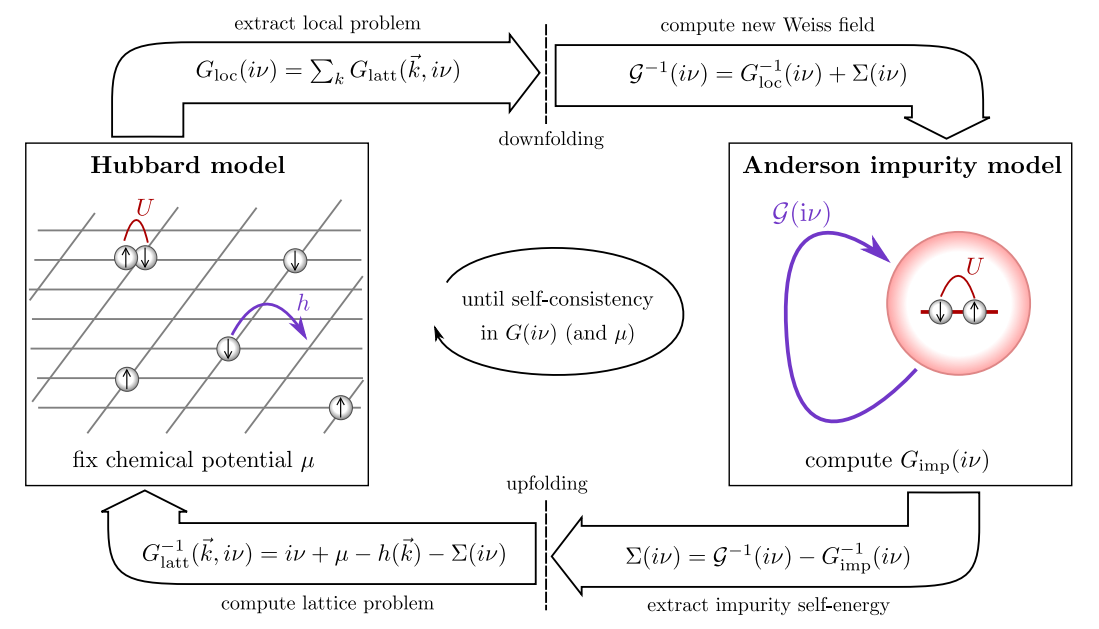
\includegraphics[width=1.0\textwidth]{figures/dmft.png}
    \caption{Self-consistency loop of dynamical mean field theory for a Hubbard-type model. Image taken from Markus Wallerberger's dissertation.}
    \label{fig:dmft}
\end{figure}

\section{Fixed-point iteration}
% TODO drop this?
% TODO define trial and result

Consider a function \(\varphi\colon M \to M\) and a starting point \(x_0 \in M\). The sequence \((x_k)_{k \in \mathbb{N}_0}\) generated by the fixed-point iteration is defined by \(x_{k+1} = \varphi(x_k)\) with \(k \in \mathbb{N}_0\).

The Banach fixed-point theorem guarantees that the sequence converges to the single fixed-point \(\varphi(x^\ast) = x^\ast\) if \(M\) is a complete metric space and \(\varphi\) is a contraction.

\section{Mixing}

Mixing is a technique to improve convergence for self-consistency iteration. The idea is to construct a more effective trial with more information than just the previous result. To be effective such a trial has to be closer to the true value which means we want to extrapolate in terms of iterations.

The simplest approach is linear mixing
\begin{equation} \label{eq:linmix}
\hat{x}_k = (1-\beta) x_k + \beta \varphi(x_k) = x_k + \beta (\varphi(x_k) - x_k)
\end{equation}
with the relaxation parameter \(\beta\).
For \(0 < \beta < 1\) we get an under-relaxation which slows down convergence in some cases, but also dampens oscillations. If the self-consistency iterations diverge, the use of under-relaxation might help out.
For \(\beta > 1\) we get over-relaxation which can have predictive behaviour and speed up the convergence but it also amplifies errors and might result in divergence.

More complex mixing techniques use trials and results of multiple previous iterations and try to combine under-relaxation for robustness and prediction to increase the rate of convergence.

\section{DIIS}
% TODO mention svd? -> maybe better for outlook

The direct inversion of the iterative subspace (DIIS), also known as Pulay mixing, is an extrapolation technique developed by Peter Pulay. His intention was to accelerate and stabelize the convergence of the Hartree-Fock self-consistent field method.\cite{diis_pulay1}\cite{diis_pulay2} % TODO dft

DIIS uses trials and results of multiple previous iterations, constructs a linear combination of them, and extrapolates a new trial for the next iteration. The coefficients are determined by a least squares optimization.

Pulay's DIIS attempts to guess a better trial by using multiple previous trials and results. The method assumes that a good approximation of the true value \(x^\ast\) can be obtained by a linear combination of the previous trials.
\begin{equation} \label{eq:diis_x}
\overline{x}_{k} = \sum_{j=0}^{m} c_j x_{k-j}
\end{equation}
where \(m\) is the number of previous trials to consider. We can also write this sum in terms of the true value \(x^\ast\) and an error vector \(e_{k} = x^\ast - x_{k}\).
\[\overline{x}_{k} = \sum_{j=0}^{m} c_j (x^\ast + e_{k-j}) = x^\ast \sum_{j=0}^{m} c_j + \sum_{j=0}^{m} c_j e_{k-j}\]
To get close to the real value \(x^\ast\) we set \(\sum_{j=0}^{m} c_j = 1\) and try to minimize the second term \(\sum_{j=0}^{m} c_j e_{k-j}\). But since we do not know the true value \(x^\ast\) we cannot know \(e_{k}\). Therefore, we approximate \(e_{k}\) by the residuals, i.e. \(e_{k} \approx f_{k} = g(x_k) - x_k\).
\[\overline{f}_{k} = \sum_{j=0}^{m} c_j f_{k-j}\]
In order to minimize \(\overline{f}_{k}\) we use the \(l^2\)-norm.

One solution would be to use the Lagrange multiplier technique to satisfy the constraint \(\sum_{j=0}^{m} c_j = 1\) and minimize \(|\overline{f}_{k}|^2\).

However, we can embed the constraint by rewriting \footnotemark
\begin{equation} \label{eq:diis_f}
\overline{f}_{k} = f_k - \sum_{j=1}^{m} \gamma_j {\Delta f}_{k-m+j} = f_k - F_k \Gamma_k
\end{equation}
with \({\Delta f}_{k} = f_k - f_{k-1}\), \(F_k = [{\Delta f}_{k-m+j}]_{j=1..m}\) and \(\Gamma_k = [\gamma_j]_{j=1..m}\).

\footnotetext{For example with \(m=2\) we get \(\overline{f}_{k} = f_k - \gamma_1 {\Delta f}_{k-1} - \gamma_2 {\Delta f}_{k}\ = f_k - \gamma_1 (f_{k-1} - f_{k-2}) - \gamma_2 (f_k - f_{k-1}) = (1-\gamma_2) f_k + (\gamma_2 - \gamma_1) f_{k-1} + \gamma_1 f_{k-2} = c_0 f_k + c_1 f_{k-1} + c_2 f_{k-2}\). Equating coefficients leads to \(\sum_{j=0}^{m} c_j = 1\).}

We minimize \(|\overline{f}_{k}|^2\) by \(\Gamma_k\) and get the solution \footnotemark
\begin{equation} \label{eq:diis_gamma}
\Gamma_k = (F_k^\dagger F_k)^{-1} F_k^\dagger f_k = F_k^+ f_k
\end{equation}

\footnotetext{The last equals is only true if \(F_k^\dagger F_k\) is invertible. The Moore–Penrose inverse exists even if that is not the case.}

Similar to \eqref{eq:linmix} we can contruct a new trial with \eqref{eq:diis_x}, \eqref{eq:diis_f} and \eqref{eq:diis_gamma}.
\begin{equation} \label{eq:diis_final}
x_{k+1} = \overline{x}_k + \beta \overline{f}_k = x_k + \beta f_k - (X_k + \beta F_k) (F_k^\dagger F_k)^{-1} F_k^\dagger f_k
\end{equation}

Variations of the DIIS method exist to further increase the rate of convergence and stability. The restarted Pulay method\cite{diis_restarted} and the periodic Pulay method\cite{diis_periodic} reset the state or use linear mixing inbetween to reduce side effects of DIIS.

% TODO least squares interpretation



\chapter{Method}
\label{ch:method}
\chapter{Method}
\label{ch:method}

\section{w2dynamic}

w2dynamics\cite{w2dyn} is a hybridization-expansion continuous-time quantum Monte Carlo package, developed jointly in Wien and Würzburg. It was written by N. Parragh, M. Wallerberger, A. Hausoel, P. Gunacker, A. Kowalski, F.Goth and G. Sangiovanni. w2dynamics contains a multi-orbital quantum impurity solver for the Anderson impurity model, a dynamical mean-field theory self-consistency loop, a maximum-entropy analytic continuation, as well as coupling to density functional theory. The dynamical mean-field theory (DMFT) self-consistency loop was in focus of this project.

\section{Cluster computing}

Since each iteration of the DMFT cycle involves a quantum Monte Carlo simulation with a high amount of measurements to get numerical stable results, w2dynamics has to be excecuted on a cluster. Most of the time was spent on the HCLM cluster with debugging and testing. The wait time is small compared to VSC-3 and the performance compareable for this specific workload.

\section{Programming language}
% TODO h5py?

w2dynamics is written two languages. The computational heavy parts are written in Fortran to get high performance. The rest, which is mostly glue code, configuration, as well as the self-consistency loop for DMFT, is written in Python for simplicity. The programming language of choice for this project was Python since a mixing template was already in place.

Besides Python and its standard library this project relied heavily on numpy as linear algebra framework and pyplot for plotting and debugging.

\section{Tools}

w2dynamic resides in a git repository at the University of Würzburg. One part of this project was to create a new branch for the DIIS mixing and to get it merged.

hgrep is a universal tool for printing and plotting outputs. It is part a of the w2dynamic repository and written in Python.



\chapter{Implementation}
\label{ch:impl}
\chapter{Implementation}
\label{ch:impl}
% TODO which files needed to be modified, change in settings
% TODO changes only necessary in python code

\section{DIIS}
% TODO linmix already existed as a starting point

\begin{lstlisting}[label=lst:diis, language=python, caption=DIIS implementation]
import numpy as np
from numpy.linalg import multi_dot

class DiisMixer(object):
  def __init__(self, oldshare, history, period):
    self.alpha = 1 - oldshare
    self.history = history
    self.period = period
    
    self.i = 0
    self.trials = []
    self.residuals = []

  def __call__(self, new_value):
    if self.i == 0:
      # no history yet
      result = new_value
    else:
      trial = self.trials[-1]
      residual = new_value - trial
      self.residuals.append(residual)
      
      # trim history
      self.trials = self.trials[:self.history]
      self.residuals = self.residuals[:self.history]
      
      if self.i <= 2 or (self.i % self.period) != 0:
        # linear mixing
        result = trial + self.alpha * residual
      else:
        # pulay mixing
        R = np.array(self.trials); R = R[1:] - R[:-1]; R = R.T
        F = np.array(self.residuals); F = F[1:] - F[:-1]; F = F.T
        result = trial + self.alpha * residual - multi_dot([
            R + self.alpha * F, np.linalg.pinv(F), residual])
        
        self.i += 1
        self.trials.append(result)
        return result
\end{lstlisting}

This DIIS mixing implementation works with real vectors. It is similar to the periodic Pulay method\cite{diis_periodic}. The most significant difference is the use of the pseudo inverse which exists if \(F_k^\dagger F_k\) is not invertible.

\section{Refactor}
% TODO why refactor and what -> mix all quantities in one step -> why
% TODO explain/cite decorator pattern and why it fits

The quantities we want to mix are not vectors but higher dimensional objects with complex numbers. To use our DIIS implementation in this case, we can naively reshape the data to a vector and seperate the real and imaginary part of the complex numbers. This functionality was implemented with the Decorator pattern.

\begin{lstlisting}[label=lst:flatdec, language=python, caption=Flat mixing decorator]
import w2dyn.auxiliaries.deepflatten as deepflatten

class FlatMixingDecorator(object):
  def __init__(self, mixer):
    self.mixer = mixer
  def __call__(self, *args):
    if len(args) == 1: args = args[0]
    types = deepflatten.types(args)
    shape = deepflatten.shape(args)
    x = deepflatten.flatten(args)
    x = self.mixer(x)
    x = deepflatten.restore(x, shape, types)
    return x
\end{lstlisting}

\begin{lstlisting}[label=lst:realdec, language=python, caption=Real mixing decorator]
import numpy as np

class RealMixingDecorator(object):
  def __init__(self, mixer):
    self.mixer = mixer
  def __call__(self, x):
    n = x.shape[0]
    x = np.concatenate([np.real(x), np.imag(x)])
    x = self.mixer(x)
    x = x[:n] + 1j*x[n:]
    return x
\end{lstlisting}

\section{Deep flatten}
% TODO why deep flatten -> input is a mix of numbers, python lists and numpy arrays with different data types -> generalization desireable to avoid input constraints (wide contract)
% TODO explain functions, mention recursion caused by nested lists

\begin{lstlisting}[label=lst:deepflat, language=python, caption=deepflatten.py]
import numbers
import numpy as np

def types(x):
  if type(x) is np.ndarray: return x.dtype
  if isinstance(x, numbers.Number): return type(x)
  result = []
  for i in x: result.append(types(i))
  return result

def shape(x):
  if type(x) is np.ndarray: return x.shape
  if isinstance(x, numbers.Number): return 1
  result = []
  for i in x: result.append(shape(i))
  return result

def flatten(x):
  if type(x) is np.ndarray: return x.flatten()
  if isinstance(x, numbers.Number): return np.array([x])
  result = np.array([])
  for i in x: result = np.append(result, flatten(i))
  return result

def restore(x, shape, types):
  def recursive(x, shape, types):
    if isinstance(shape, tuple):
      size = np.prod(shape)
      return x[:size].reshape(shape).astype(types), size
    if shape == 1:
      return types(x[0]), 1
    result = []
    offset = 0
    for s, t in zip(shape, types):
      tmp = recursive(x[offset:], s, t)
      result.append(tmp[0])
      offset += tmp[1]
    return result, offset
  return recursive(x, shape, types)[0]
\end{lstlisting}



\chapter{Evaluation}
\label{ch:evaluation}
\chapter{Evaluation}
\label{ch:evaluation}
The hclm cluster was used to evaluate the usability and performance of DIIS for mixing the self-energy. We decided to use reasonably small calculations that would finish in a few hours.

For each testing, we considered a square-lattice Hubbard model at interaction $U=8t$ and temperature $T=t/50$, where $t$ is the hopping amplitude.

\lstdefinelanguage{ini}{
  basicstyle=\ttfamily\small,
  columns=fullflexible,
  morecomment=[s][\color{Orchid}\bfseries]{[}{]},
  morecomment=[s][\color{Orchid}\bfseries]{[[}{]]},
  morecomment=[l]{\#},
  morecomment=[l]{;},
  commentstyle=\color{gray}\ttfamily,
  morekeywords={},
  keywordstyle={\color{green}\bfseries}
}

\begin{lstlisting}[label=lst:w2dyn_config, language=ini, caption=The w2dynmaics configuration for this case]
[General]
DOS=ReadIn
HkFile=hubbard_2d_80_80_1.hk
beta=50.
NAt=1
totdens=1.
EPSN=0
mu=4.0
DMFTsteps=50
StatisticSteps=0
FileNamePrefix=square_u08_b50_diis
magnetism=para
siw_moments=estimate
FTType=none
mixing=0.0
mixing_strategy=diis
mixing_diis_history=5
mixing_diis_period=1

[Atoms]
[[1]]
Hamiltonian=Density
Udd=8.0
Nd=1

[QMC]
Nwarmups=1e6
Nmeas=1e5
NCorr=200
Ntau=1000
Niw=2000
Eigenbasis=1 
MeasGiw=1
\end{lstlisting}

The reference was given by the same configuration, but without DIIS mixing. It was important to compare the results with and without DIIS to see if they agree. Different results would be a hint to a bug in the implementation or that DIIS is not applicable for these inputs or DMFT in general. The configuration file is given in listing \ref{fig:eval-diis-u8}.

\begin{figure}[H]
    \centering
    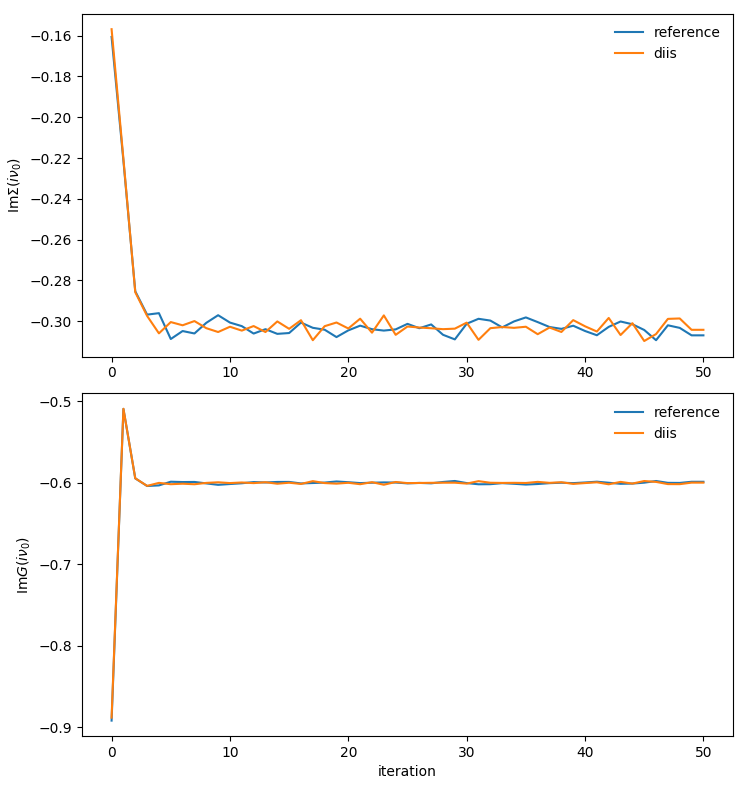
\includegraphics[width=1.0\textwidth]{figures/square_u08_b50_siw_imag_giw_imag.png}
    \caption{DMFT iteration comparison for Matsubara frequency $\pi/\beta$ and $U=8t$}
    \label{fig:eval-diis-u8}
\end{figure}

\begin{figure}[H]
    \centering
    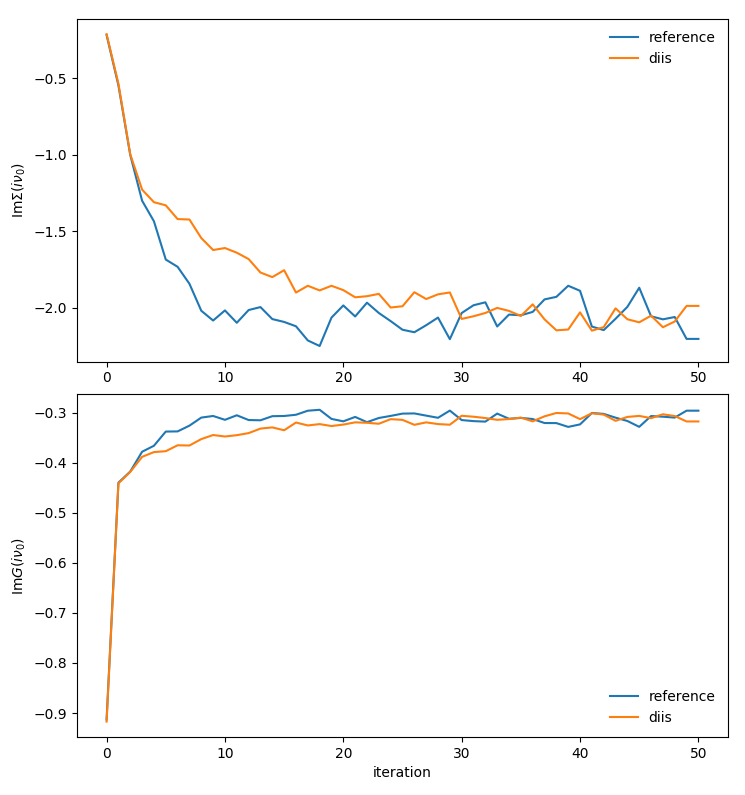
\includegraphics[width=1.0\textwidth]{figures/square_u12_b50_siw_imag_giw_imag.png}
    \caption{DMFT iteration comparison for Matsubara frequency $\pi/\beta$ and $U=12t$}
    \label{fig:eval-diis-u12}
\end{figure}

We can see that in figure \ref{fig:eval-diis-u8} that the result is the same with and without mixing while the rate of convergence is very similar.

A higher $U$ in figure \ref{fig:eval-diis-u12} shows a slower convergence in case of DIIS while the result is still the same. We are assuming that this is caused by the QMC noise. The DIIS appears to suppress this noise. A recent implementation of symmetric improved estimators\cite{symmetric} by Josef Kaufmann is promising better performance with DIIS.



\chapter{Conclusion}
\label{ch:conclusion}
\chapter{Conclusion}
\label{ch:conclusion}
% TODO noise might be a problem for DIIS (comparing qmc vs symmetry thing)
% TODO -> weighted least squares to handle qmc noise
% TODO anderson mixing? ml mixing?



\chapter{Outlook}
\label{ch:outlook}
\chapter{Outlook}
\label{ch:outlook}
% TODO drop this?



\cleardoublepage
\pagenumbering{roman} \setcounter{page}{1}
\printbibliography

\end{document}
